\section{训练过程诊断}
\label{sec:training-diagnostics-appendix}

图\ref{fig:training-dynamics}记录QDPT在PathVQA上的三次完整训练。三条日志损失曲线接近，但Prompt范数、Workspace表示尺度和视觉注意力熵在训练中逐渐分离。该现象与最终准确率的运行间差异同时出现，不过这些轨迹不能单独确定差异来自哪个模块。

\begin{figure}[htbp]
    \centering
    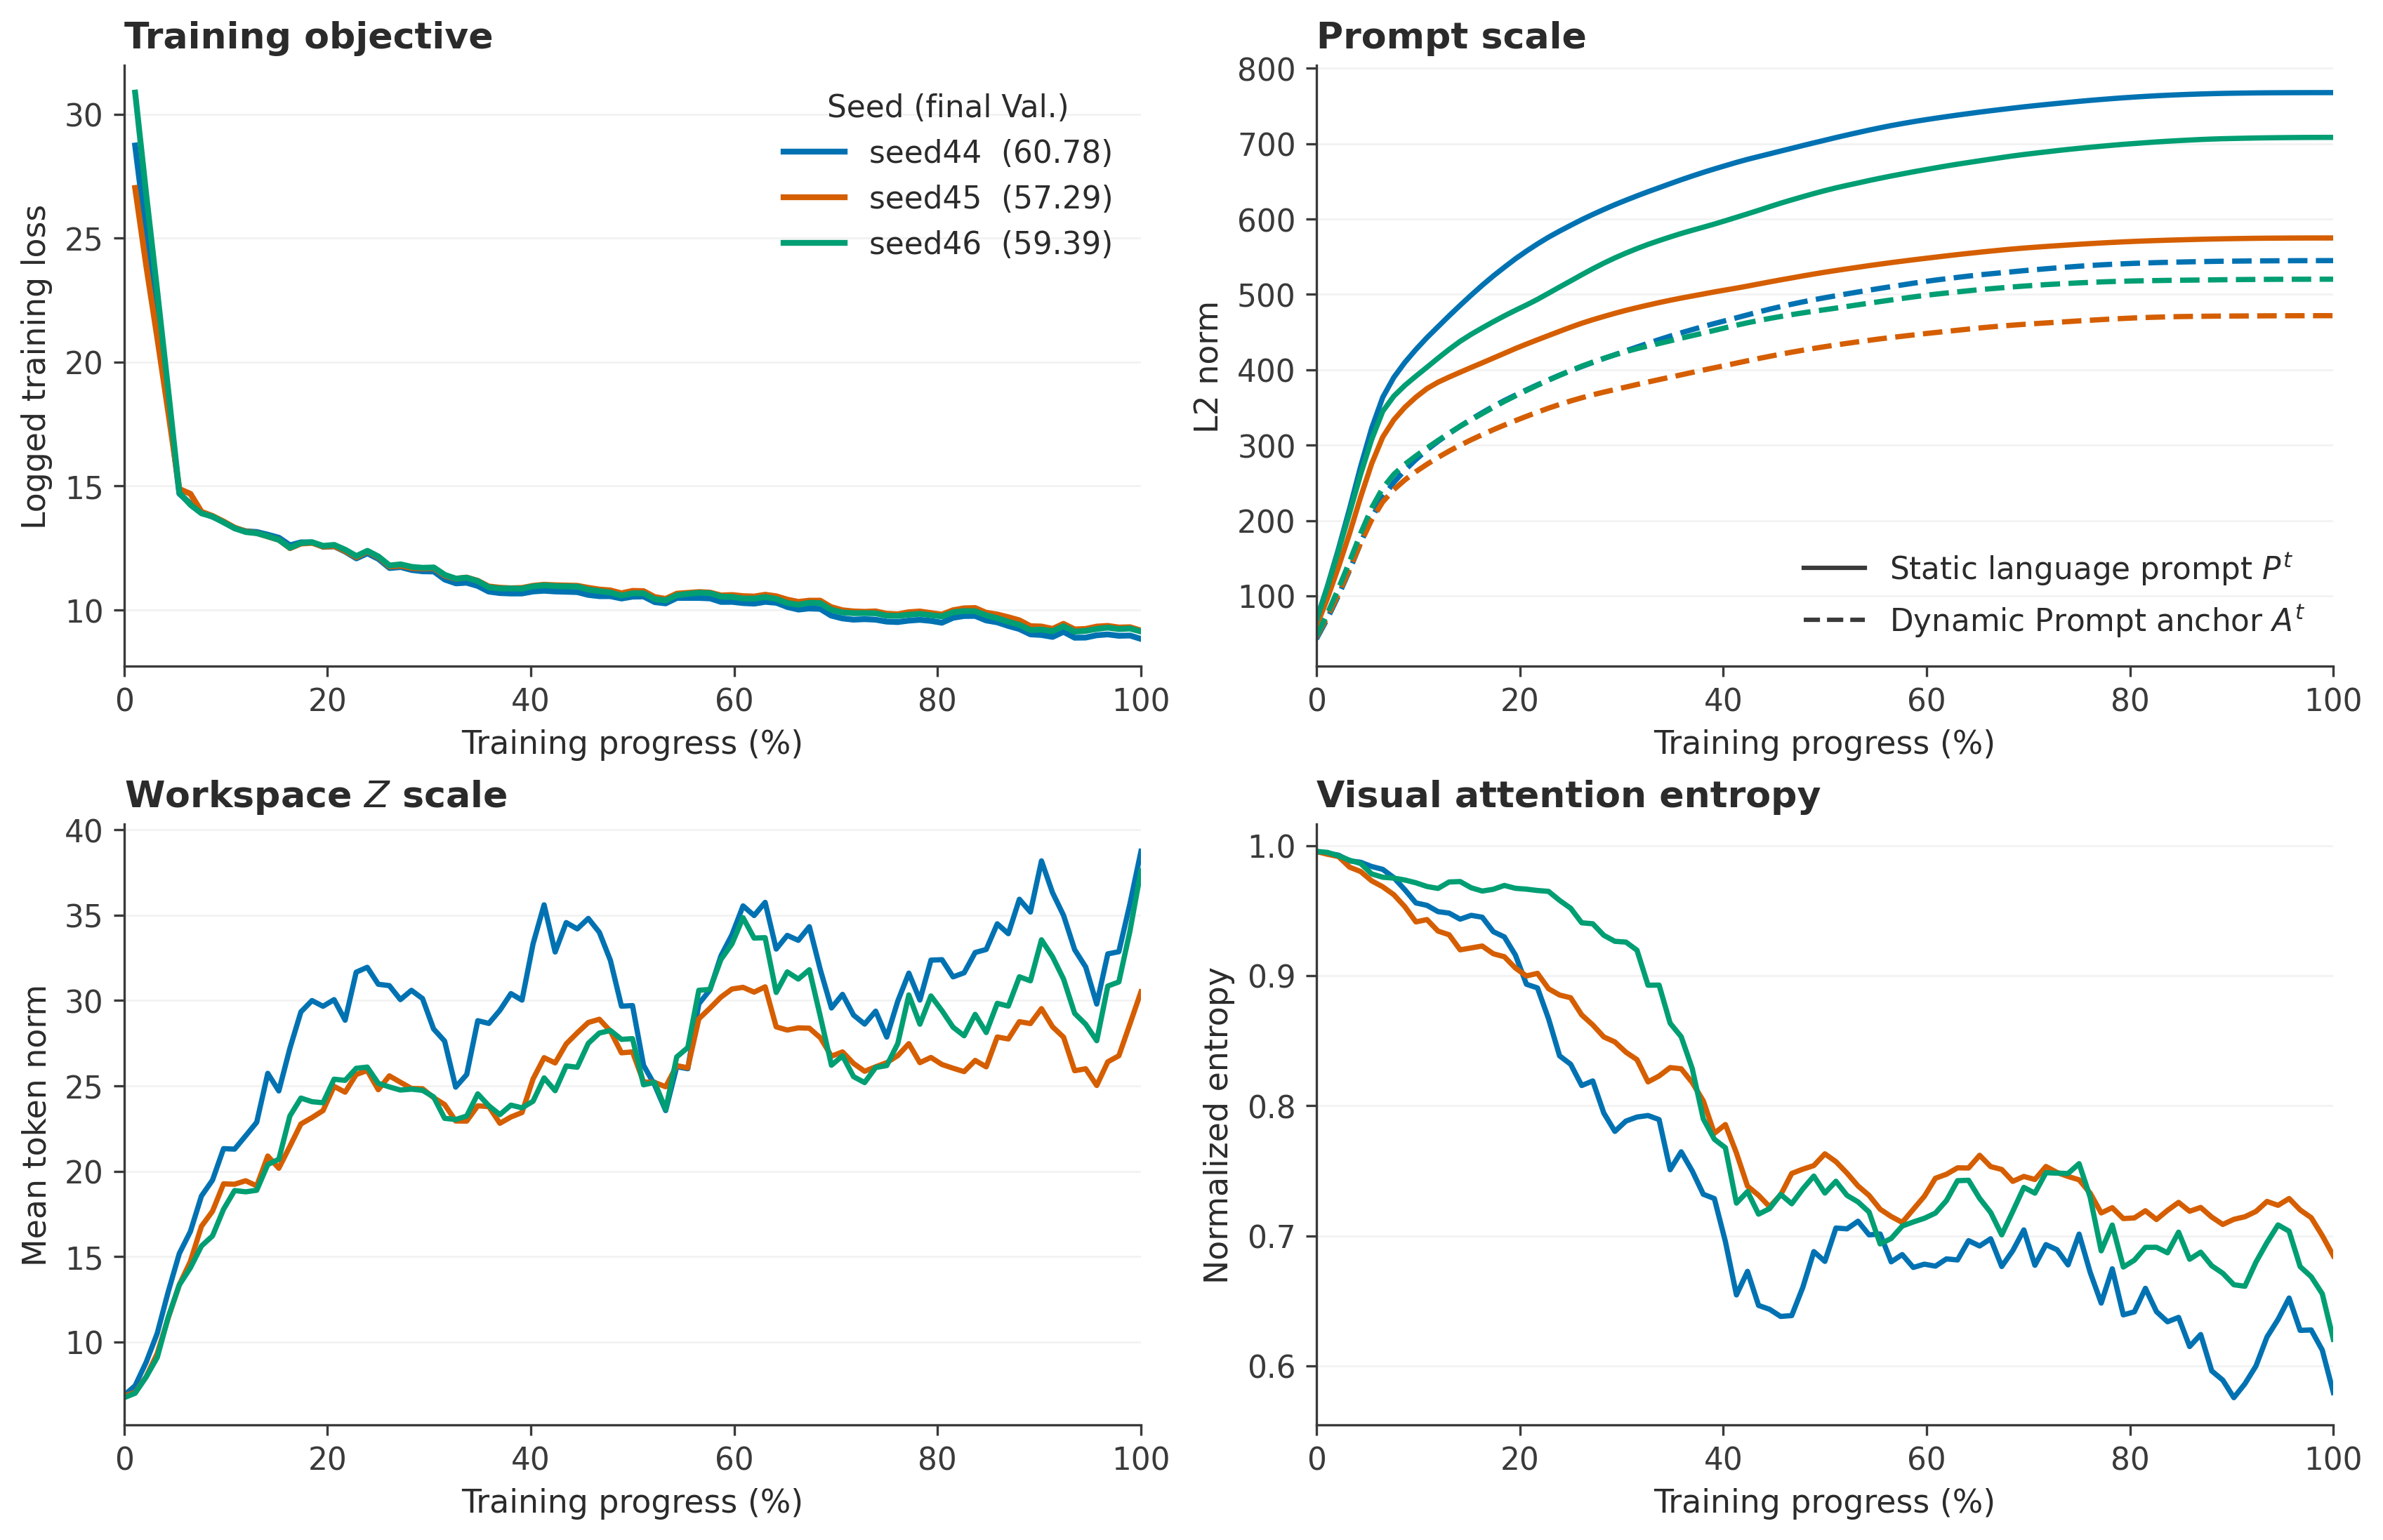
\includegraphics[width=\textwidth]{figures/qdpt_training_dynamics.png}
    \caption{QDPT在PathVQA上的三随机种子训练轨迹。训练器每20个优化器步记录一次区间平均损失，图中各曲线采用7点滑动平均；横轴按各次运行的记录步数归一化。右上图的实线与虚线分别表示静态语言Prompt $P^t$和文本Anchor的$L_2$范数。视觉注意力熵先以有效视觉Token数的对数归一化，再对batch、注意力头和Query槽取平均。}
    \label{fig:training-dynamics}
\end{figure}
